\documentclass{article}
\usepackage[utf8]{inputenc}
%\usepackage [danish]{babel} % Vi burde ikke have brug for den her
\usepackage[a4paper, hmargin={2.8cm, 2.8cm}, vmargin={2.5cm, 2.5cm}]{geometry}
\usepackage{eso-pic} % \AddToShipoutPicture
\usepackage{graphicx} % \includegraphics
\usepackage{import}
\linespread{1.2}
\usepackage{pbox}
\usepackage{amsthm}
\usepackage{amsmath}
\usepackage{url}
\usepackage{tikz}
\usepackage{amsfonts}
\usepackage{standalone}
\newtheorem{theorem}{Teorem}
\newtheorem{lemma}{Lemma}
\newtheorem{korollar}{Korollar}

\newtheorem{mydef}{Definition}
\newtheorem{myex}{Example}
\usepackage{caption}
\DeclareMathOperator*{\argmin}{arg\,min}

\author{
\huge{Supervisors}\\
\Large{Rasmus Fonseca}\\
\Large{Niels Bjørn Bugge Grathwohl}\\
\Large{Ulrik Rasmussen}\\
    \\ \texttt{}
}

\title{
  \vspace{3cm}
  \Huge{Genome pattern matching using regular expressions} \\
  \Large{Simon Nicolai Lefoli Maibom - xvm226} \\
  \Large{Arinbjörn Brandsson - hkt789}\\
  \Large{Martin Simon Haugaard - cdl966}
}

\usepackage{natbib}
\usepackage{graphicx}

\newcommand{\myfl}{\left\lfloor}
\newcommand{\myfr}{\right\rfloor}
\newcommand{\mycl}{\left\lceil}
\newcommand{\mycr}{\right\rceil}

\begin{document}

%% Change `ku-farve` to `nat-farve` to use SCIENCE's old colors or
%% `natbio-farve` to use SCIENCE's new colors and logo.
\AddToShipoutPicture*{\put(0,0){\includegraphics*[viewport=0 0 700 600]{lib/natbio-farve}}}
\AddToShipoutPicture*{\put(0,602){\includegraphics*[viewport=0 600 700 1600]{lib/natbio-farve}}}

%% Change `ku-en` to `nat-en` to use the `Faculty of Science` header
\AddToShipoutPicture*{\put(0,0){\includegraphics*{lib/nat-en}}}

\clearpage\maketitle
\thispagestyle{empty}

\newpage

\tableofcontents
 
\newpage

\section{Introduction}

\section{Preliminaries}
\section{Deoxyribonucleic and Ribonucleic Acids}
Deoxyribonucleic acids (DNA) and ribonucleic acids (RNA), collectively known as 
nucleic acids, are one of the three 
essential molecules for life, the last two being proteins and carbohydrates. 
DNA creates RNA through transcription and RNA creates proteins through 
translation, while proteins performs a variety of tasks, one 
of which is packaging and controlling the long DNA molecules~\cite[p. 172]{alberts}. 
In this section we will briefly detail the functions of DNA and RNA as well as their 
secondary structure.
\subsection{DNA}
Deoxyribonucleic acid (DNA) is a macro molecule composed of nitrogenous bases 
joined by deoxyribose-phosphate into long strands. One nitrogenous base which 
is joined with a sugar\footnote{Deoxyribose or ribose}-phosphate is called a 
nucleotide. DNA can have four nitrogenous bases:
\begin{itemize}
\item Guanine (G)
\item Adenine (A)
\item Cytosine (C)
\item Thymine (T)
\end{itemize}
DNA is primarily found in nature as helixes, where two strands have bonded. Each 
base has a complementary base with which they can form a hydrogen bond. 
G is the complementary base of C and A is the complementary base of T.

DNA holds the hereditary material of the cells and can replicate itself by 
detaching two bonded strands, then use each as a template for a new strand 
to bond with the detached strands~\cite[p. 199]{alberts}.
\subsection{RNA}
Ribonucleic acid (RNA) is a macro molecule composed of long strands of 
nucleotides. RNA have the same nitrogenous bases as DNA except for T, which is 
changed during transcription from DNA to RNA into Uracil (U) which bonds with 
A. In nature, the predominant form of RNA are as single-stranded chains that 
can fold back on themselves or bundled with other chains to form a structure. This 
flexibility of the backbone, which allows for chains to fold in on themselves is 
possible because the RNA's backbone is composed of a sugar called ribose, which 
allows more flexibility compared to its alternative form, deoxyribose, used in 
deoxyribonucleic acid (DNA).

%Maybe delete next part
When DNA creates RNA through transcribing portions of its sequence\footnote{A 
sequence is a succession of nucleotides}, five different kinds of RNA are 
created. Three are responsible for protein synthesis which allows for the creaiton 
of proteins, one is for regulating the DNA's gene expression, and the last 
is used for miscellaneous functions\cite[p. 236, table 7-1]{alberts}.
\subsection{Secondary Structure}\label{structs}
The secondary structure of DNA and RNA describes how bases of 
strands bond to themselves. The secondary structure can change if 
a strand is damaged or has mutated, causing it to gain or lose 
bases. Below are examples of three common secondary structures.

\subsubsection{Bulge}
A bulge occurs when one or more bases have no base to bond with, and these 
bases are surrounded by bases which have bonded. This causes the bases to get 
pushed out slightly, resembling a bulging growth. This type of structure occurs 
when one or more bases has been inserted or deleted. If a base has been 
inserted it will have no base to bond with, and if a base has been deleted 
the previously-bonded base will have no base to bond with. Figure~\ref{fig:bulge} shows a bulge.

\begin{figure}[H]
\centering
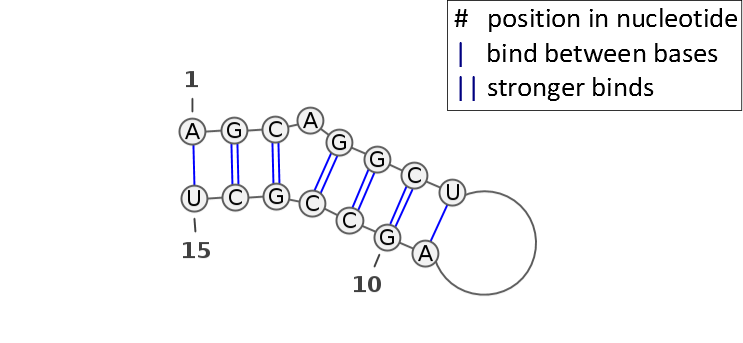
\includegraphics[scale=0.4]{./lib/bulge.png}
\caption{The RNA sequence {\tt AGCAGGCUAGCCGCU}. Note the bulging {\tt A} at position 4.}
\label{fig:bulge}
\end{figure}~
\\
\subsubsection{Interior Loop}
An interior loop occurs when two or more opposing bases are not complementary and 
can not bond, causing them both to bulge. This occurs when one or more 
consecutive bases mutate to another base. Figure~\ref{fig:int-loop} shows an interior 
loop.
\begin{figure}[h!]
\centering
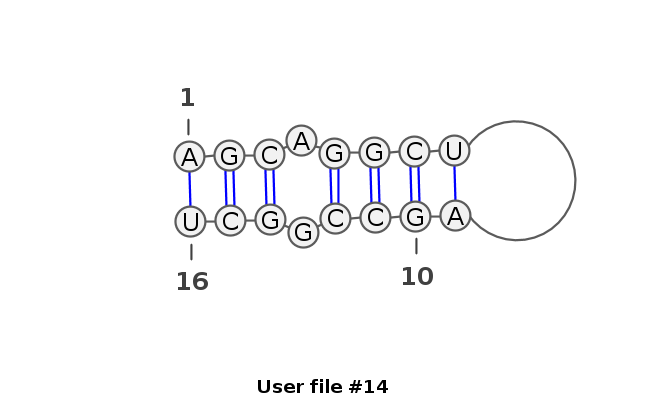
\includegraphics[scale=0.4]{./lib/interior-loop.png}
\caption{The RNA sequence {\tt AGCAGGCUAGCCGGCU}. Note the bulging {\tt A} at position 4 and {\tt G} at position 13
creating a loop inside the bonded strand.}
\label{fig:int-loop}
\end{figure}\\
These interior loops vary in size, and can have differing amount of bases on 
either side of the strands.
\subsubsection{Stem Loop}
A stem loop, also known as a hairpin loop, occurs when a strand bonds with 
itself, but leaves a sequence of bases sticking out, which does not bond with anything. 
This kind of loop occurs typically in RNA as they are single-stranded, but may 
happen in single stranded DNA. Figure~\ref{fig:stem-loop} 
shows a stem loop.
\begin{figure}[h!]\centering
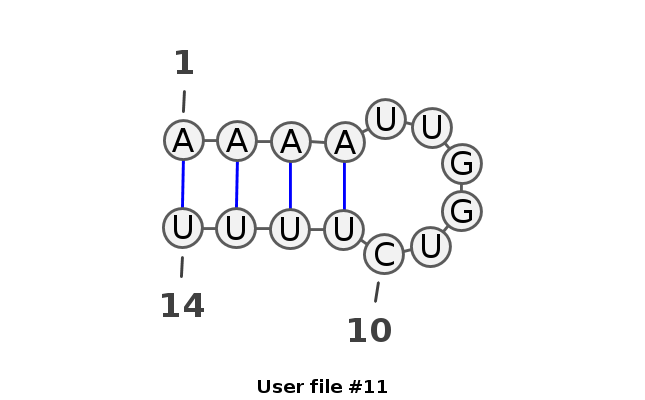
\includegraphics[scale=0.35]{./lib/stem-loop.png}
\caption{A stem loop of the RNA sequence {\tt AAAAUUGGUCUUUU}.}
\label{fig:stem-loop}
\end{figure}\\
An important thing to note is how the sequence can be seen as one 
long strand that starts from the adenine bases, which binds with the uracil bases, 
loops around without binding to anything and finally become the uracil bases 
which binds with the adenine bases from the beginning. This means that the 
stem loop from Figure~\ref{fig:stem-loop} can be written as one continuous 
sequence of bases; {\tt AAAAUUGGUCUUUU}. Since we can define a stem loop, we can 
search through a file documenting the bases of a nucleic acid and find all stem 
loops.

\documentclass[11pt,twoside,a4paper]{article}
\usepackage{pbox}
\usepackage{amsthm}
\newtheorem{definition}{Definition}
\newtheorem{example}{Example}
\begin{document}
\subsection{Scan\_For\_Matches}
Scan\_for\_matches is a string-searching tool created by Ross Overbeek, David 
Joerg and Morgan Price in C which searches through FASTA text files. Users specify 
what they wish to search for by defining a pattern, and scan\_for\_matches 
returns all matches that corresponds to the specified pattern.
\begin{definition}\label{patd}
A pattern is defined as follows:\\
\begin{tabular}{|r|l|}
\hline
{\tt ACUG}&Match the sequence ACUG\\
\hline
{\tt 1...5}&Match 1 to 5 characters\\
\hline
{\tt 3...3}&Match exactly 3 characters\\
\hline
{\tt p1=1...5}&Match 1 to 5 characters, and call the sequence p1\\
\hline
{\tt p1 $|$ p2}&Match either p1 or p2\\
\hline
{\tt p1[1,0,0]}&Match p1, allowing for one mismatch\\
\hline
{\tt p1[0,1,0]}&Match p1, allowing for one deletion\\
\hline
{\tt p1[0,0,1]}&Match p1, allowing for one insertion\\
\hline
{\tt length(p1+p2) $<$ 5}&The combined length of p1 and p2 must not exceed 4\\
\hline
{\tt r1=\{AB, BA\}}&\pbox{20cm}{Create a pattern rule where A is the complement of B, \\and B is the complement of A, and call it r1}\\
\hline
{\tt $<$p1}&Match the reverse of p1\\
\hline
{\tt \textasciitilde p1}&\pbox{20cm}{Match the reverse complement of p1 using the G-C, \\C-G, A-T and T-A pairing rule}\\
\hline
{\tt r1\textasciitilde p1}&\pbox{20cm}{Match the reverse complement of p1 using r1 rules}\\
\hline
{\tt \textasciicircum ~p1}&\pbox{20cm}{Match only p1 if it is at the start of a string}\\
\hline
{\tt p1 \$}&Match only p1 if it is at the end of a string\\
\hline
\end{tabular}
\end{definition}

\begin{definition}\label{patc}
Let {\tt E} be any pattern that's in the alphabet $\Sigma$ as defined in Definition \ref{patd}. 
Let $\epsilon$ be the empty string.
Let {\tt A} be a string that we are processing to see if the pattern is valid.
A pattern may then be constructed as such: \begin{center}
{\tt A = A' A | $\epsilon$}\\
{\tt A' = E}\end{center}
\end{definition}
Definition \ref{patc} states that a pattern may be any combination of the alphabet 
defined in definition \ref{patd}.
Using these patterns, it is possible to make very specific or very broad 
searches in a text file. 

\begin{example}
Say we want to write a pattern that finds the sequence {\tt GUUC}, allowing 
one mismatch, followed by a random sequence which has a length between 3 and 5, 
followed by the reverse complement of the first sequence that we found. We can 
then write this as \begin{center}
{\tt p1=GUUC[1,0,0] 3...5 \textasciitilde p1}
\end{center}
\end{example}

\end{document}

\section{Theory}

\section{Method}

\section{Conclusion}





\end{document}
